\documentclass{article}
\usepackage[hidelinks]{hyperref}
\usepackage{Sweave}
\begin{document}
\input{FindingSeedTraps-concordance}

\title{Finding Seed Traps In USGS Plots}
\author{Samantha Davis}

\maketitle

\section{Introduction}
I made a series of functions that will rotate ``crooked'' plots and draw subplot lines for those plots, to generate corners. These subpolygon corners are needed by the function TrapUTM, generated by Danielle and Carrie. This PDF will introduce the use of those functions and hopefully, barring any weird or bad data, we can generate seed trap locations for any plots of interest.

\section{Loading the Package and Data}
I used ``BBBPIPO'' as my sample plot, simply because it was at the top of the list. Now, you'll need to have a few data files loaded into R. I've saved the individual trees file as treeinfo, the seedling counts as seedlings, and the plot descriptions as plotinfo. I'll load these locally and do a head() command so that you can see:

\begin{Schunk}
\begin{Sinput}
> load("../data/plotinfo.RData")
> load("../data/seedlings.RData")
> load("../data/treeinfo.RData")
> head(plotinfo)
\end{Sinput}
\begin{Soutput}
         Plot Park Elev     UTME    UTMN size_ha sdl_pl BA_m2_ha  Est Burn Sdl.
1    YOHOPIPO YOSE 1500 247367.0 4187650     1.0      2     76.4 1991 2007    1
2     BBBPIPO SEKI 1609 339876.0 4048133     1.0      2     66.5 1992 <NA>    1
3     CCRPIPO SEKI 1637 338884.0 4048723     1.1      2     68.3 1991 <NA>    1
4    CRCRPIPO YOSE 1637 255941.6 4179572     1.0      2     77.8 1993 <NA>    1
5 FFS7CONTROL <NA> 1941 342286.0 4049870     1.0      .        . 2001 <NA>    1
6    FFS6BURN <NA> 2018 342588.0 4050299     1.0      .        . 2001 2003    1
  Clim99_08. Adults. ABCO ABMA CADE PICO PIJE PILA PIMO PIPO PSME QUCH QUKE
1          1       1   35    0   32    0    0   26    0    5    1    0    1
2          1       1   12    0   55    0    0    5    0    4    0    1   24
3          1       1   46    0   30    0    0    5    0    4    0    0   15
4          1       1   44    0   29    0    0   19    0    6    0    0    2
5          0       1    .    .    .    .    .    .    .    .    .    .    .
6          0       1    .    .    .    .    .    .    .    .    .    .    .
  SEGI            Forest X
1    0     Mixed conifer  
2    0     Mixed conifer  
3    0     Mixed conifer  
4    0     Mixed conifer  
5    . White fir - mixed  
6    . White fir - mixed  
\end{Soutput}
\begin{Sinput}
> head(seedlings)
\end{Sinput}
\begin{Soutput}
  PLOT_NAME SUBPLOT QUADRAT SPPCODE SIZE_CLASS COUNT1999 COUNT2000 COUNT2001
1   BBBPIPO       6       1    ABCO          1         0         0         0
2   BBBPIPO       6       1    ABCO          2        62        26         0
3   BBBPIPO       6       1    ABCO         10         0         4        28
4   BBBPIPO       6       1    CADE          1         0         4         0
5   BBBPIPO       6       1    CADE          2         6         1         0
6   BBBPIPO       6       1    CADE         10         4         9         6
  COUNT2002 COUNT2003 COUNT2004 COUNT2005 COUNT2006 COUNT2007 COUNT2008
1         0         0         0         0         0         0         0
2         2         1         2         1         0         0         2
3        19        19        10         6         4         5         3
4         0        21         0        36         3        16         0
5         6         0         0         0         0         1         1
6         0         5         3         1         2         2         1
  COUNT2009 DATA_YEAR
1         5      2009
2         0      1999
3         2      2000
4         0      2000
5         0      1999
6         1      1999
\end{Soutput}
\begin{Sinput}
> head(treeinfo)
\end{Sinput}
\begin{Soutput}
     PLOT SUBPLOT TAGNUMBER SppCode IngrowthYear YearFirstRecorded
1 BBBPIPO       1      1991    ABCO           NA              1992
2 BBBPIPO       1      2012    ABCO           NA              1992
3 BBBPIPO       1      2015    ABCO           NA              1992
4 BBBPIPO       1      2022    ABCO           NA              1992
5 BBBPIPO       1      1954    CADE           NA              1992
6 BBBPIPO       1      1955    CADE           NA              1992
  MortalityYear  DBH1  DBH2  DBH3  DBH4  DBH5 DBH6 DBH7   XCoord  YCoord
1            NA   4.4   5.0   5.6   6.0   6.2   NA   NA 339902.5 4048132
2            NA   8.7   9.1   9.8  10.4  11.1   NA   NA 339908.8 4048134
3            NA   5.1   5.5   5.5   3.5   6.0   NA   NA 339908.2 4048137
4            NA   3.2   2.9   3.3   4.0   4.9   NA   NA 339905.2 4048131
5            NA 106.6 106.1 107.5 106.0 106.4   NA   NA 339882.4 4048139
6            NA  31.1  32.7  34.9  38.0  40.3   NA   NA 339887.7 4048137
\end{Soutput}
\end{Schunk}

As you can see, these are more or less unchanged from the original data files. We'll also need one more piece. I've been trying to put functions that I create into R packages for reusability. These R packages, so far, are \textit{not} on CRAN, but I do upload the packages to my GitHub. The package "devtools" in R has a neat little tool that allows you to install a package directly from GitHub. Uncomment the lines that you need, below, to install packages and download my package, nicknamed "disperseR" -- this will give you the functions to rotate plots.

\begin{Schunk}
\begin{Sinput}
> #install.packages("devtools")
> library(devtools)
> install_github("ecology-rocks/disperseR")
> library(disperseR)
\end{Sinput}
\end{Schunk}

Okay. So, I'll paste the code for each function into the end of this PDF; but you can also access the code by typing the name of the function directly into the R console. So, if something isn't working, you can try to modify it, or at least see how it works and how you might change your inputs. This package is a work in progress, and I'll be trying to update it daily, so if you access it later, you can always redownload and install from GitHub.

Because it's on GitHub, you can also download the source and try to add your own updates and documentation. You can click \href{http://hilaryparker.com/2014/04/29/writing-an-r-package-from-scratch/}{here} to get a bare-bones introduction to writing packages, and RStudio is an IDE that helps tremendously by streamlining both the package building and GitHub sharing process.

Finally, if you have a question about how to use a function in disperseR, you can access the function's help file by using the standard help feature, ?function in R. You can also do this with any data included.

Okay, onto the real code.

\section{Rotating The Plot}

Given the TrapUTM() function, we have a working, repeatable algorithm to find seed trap locations, as long as the plots are situated so that their sides are parallel with the four cardinal directions. Unfortunately, not all of the plots are situated in that fashion. BBBPIPO, for example, is in more of a "diamond" shape when you plot it. So, the first thing I did was to write a series of functions that take the plot, and its southwestern corner (found in plotinfo), and rotates it so that its southernmost point in the original plot will have the same y (North/South) value as the southwestern corner.

To do this, I found the angle of rotation, converted the points from a Cartesian system (x,y) to a Polar system (distance, angle), added the angle of rotation to each of the angles, then converted the points back to a Cartesian system. Since this rotation makes the UTMN/UTME points essentially useless, I have the new origin (southwest corner) set to (0,0), but it could be easily set to something else with the function's flexibility. Here's how it works:

\begin{Schunk}
\begin{Sinput}
> ## separate out bbbpipo
>   bbbpipo <- treeinfo[treeinfo$PLOT=="BBBPIPO",]
>   colnames(bbbpipo) <- c("plot", "subplot", "tag", "spp",
+                          "ingrowth", "firstrec", "deathyear", "dbh1",
+                          "dbh2", "dbh3", "dbh4", "dbh5",
+                          "dbh6", "dbh7", "x", "y")
> ## pull out the plot origin from plotinfo
> bbbpipoOrigin <- data.frame(x=plotinfo[plotinfo$Plot=="BBBPIPO", "UTME"],
+                             y=plotinfo[plotinfo$Plot=="BBBPIPO", "UTMN"],
+                             stringsAsFactors=FALSE)
> ## In this example, you can rotate the plot and set the origin to the trueSW
> ## values. I'm doing it this way to show how the plot is rotated. This function
> ## takes your large tree dataframe (bbbpip), and your "true southwestern corner"
> ## coordinates as a vector.
> rotateBBB <- rotatePlot(bbbpipo, truesw=c(bbbpipoOrigin[1,1], bbbpipoOrigin[1,2]), origin=c(bbbpipoOrigin[1,1], bbbpipoOrigin[1,2]))
> ## check our work
> plot(rotateBBB$x, rotateBBB$y, xlim=c(min(rotateBBB$x), max(bbbpipo$x)), ylim=c(min(bbbpipo$y), max(rotateBBB$y)), col="red", pch=4)
> points(bbbpipo$x, bbbpipo$y, col="black", pch=2)
> ## Let's overwrite rotateBBB and let the origin be the default, c(0,0), for ease
> ## of reading and seeing later on. This is just changing the values of (x,y) by
> ## a uniform amount.
> rotateBBB <- rotatePlot(bbbpipo, truesw=c(bbbpipoOrigin[1,1], bbbpipoOrigin[1,2]))
\end{Sinput}
\end{Schunk}
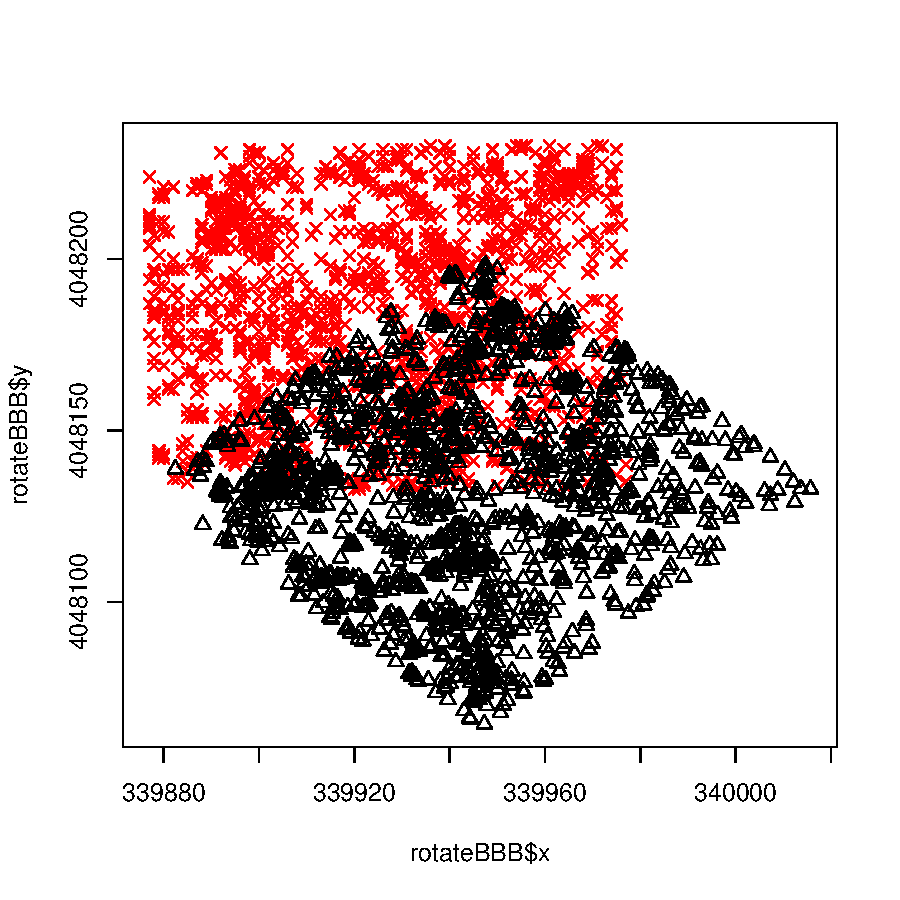
\includegraphics{FindingSeedTraps-003}

Let's check and make sure that our rotated plot is the correct size. According to the plotinfo file, it should be about a hectare or 100mx100m.

\begin{Schunk}
\begin{Sinput}
> ## set our min and max values
> corners <- c(min(rotateBBB$x),
+              max(rotateBBB$x),
+              min(rotateBBB$y),
+              max(rotateBBB$y))
> ## make sure the plot is actually 100x100
> corners[2]-corners[1]
\end{Sinput}
\begin{Soutput}
[1] 100
\end{Soutput}
\begin{Sinput}
> corners[4]-corners[3]
\end{Sinput}
\begin{Soutput}
[1] 100
\end{Soutput}
\end{Schunk}

Okay. We know the plot is 100x100, and we know the subplot file originally used had the important columns: "Subplot", "POINT\_X", and "POINT\_Y". So, we need to replicate that. Let's build all of the corners, then look in the middle for a subplot identity. First, we're going to use the function "getSubplotCoords", which basically returns a vector of values, by 25m increments, until all possible points are surrounded. So, if you have 100 m of possible points, this function will return a vector of c(0, 25, 50, 75, 100), taking into account your min(x) and max(x). This particular rotation has the x-values starting at 1 and the y values starting at 0, so we'll get back vectors of c(1, 26...101) and c(0, 25...100). I wrote it as a function so that if we have rectangular plots, it'll work just the same.

\begin{Schunk}
\begin{Sinput}
> ## get coords
>   xcoords <- getSubplotCoords(corners[1:2], increment=25)